% !TeX root = ../main.tex
% Add the above to each chapter to make compiling the PDF easier in some editors.

\chapter{Symmetries of Neural Network Weights}\label{section:geometry_of_nns}

Symmetries in data, such as rotation symmetries in molecules or translation symmetries in images, can be used to obtain useful inductive biases for ML models \citep{bronsteinGeometricDeepLearning2021,weilerEquivariantCoordinateIndependent2023}. By restricting the search space to functions that respect those symmetries, such inductive biases make training more data-efficient \citep{brehmerDoesEquivarianceMatter2024}. Since our data modality is neural network weights, taking the symmetries of neural networks into account can likewise make learning in weight space more effective. 

\begin{figure}[t!]
    \missingfigure[figwidth=\linewidth, figheight=6cm]{Diagram with permutation and scaling symmetries.}
    \caption{\label{fig:nn_sym} Symmetries of neural networks.}    
\end{figure}

Given a neural network $f$ with parameters $\theta$, we define a \textit{symmetry} as an operation $\phi$ that leaves the function computed by the neural network unchanged; i.e. $f_{\phi(\theta)}(x) = f_\theta(x)$. We are further interested only in the static symmetries that hold for any $\theta$ and thus can more reliably be used as inductive biases, rather than dynamic symmetries specific to a certain value of $\theta$. Such symmetries of neural network weights have been studied for a long time \citep{hecht-nielsenALGEBRAICSTRUCTUREFEEDFORWARD1990}, and are still key considerations for understanding the loss landscape and training dynamics of neural networks \citep{breaWeightspaceSymmetryDeep2019a,simsekGeometryLossLandscape2021,limEmpiricalImpactNeural2024,zhaoIMPROVINGCONVERGENCEGENERALIZATION2024}.

\section{Permutation and Scaling Symmetries of Neural Networks} \label{sec:perm_and_scale_sym}

A typical neural network with non-linear activations has two main kinds of symmetries: \textit{permutation symmetries} and \textit{scaling symmetries}. Permutation symmetries arise from the connectivity structure of the neural network, and scaling symmetries mainly arise from the particular non-linearities. 

More formally, consider a two-layer MLP with weight matrices $\W_1, \W_2$ and element-wise activations $\sigma$; i.e. $f_\theta(x) = \W_2 \sigma (\W_1x)$, ignoring the biases for simplicity but the following discussion applies to the biases as well. Let $\bP$ be an arbitrary permutation matrix. We can permute the hidden neurons, and apply the same permutation to their outgoing weights as well to keep the function unchanged:
\begin{equation}
    f_\theta(x) = \W_2 \sigma (\W_1x) = \W_2 \bP^T \sigma (\bP \W_1x).
\end{equation}
Since $\sigma$ is applied element-wise, we have $\W_2 \bP^T  \bP \sigma (\W_1x)$ which preserves the function as $\bP^T  \bP = \mathbf{I}$. Similarly, convolutional neural networks' channels can be permuted while preserving the function. More generally, \citet{limGraphMetanetworksProcessing2023} show that the permutation symmetries of any neural network correspond to graph automorphisms of its neural DAG, constructed with each edge corresponding to a parameter (e.g. directly the computational graph for MLPs, or with each filter corresponding to a node for CNNs).

In addition to these permutation symmetries, element-wise activation functions such as ReLU introduce further scaling symmetries to neural networks. For example, for the ReLU activation it holds for any real number $\lambda > 0$ that $\text{ReLU}(\lambda x) = \lambda \text{ReLU}(x)$. This means the input weights to a layer with ReLU activations can be multiplied with a positive number, and the function will remain unchanged as long as the output weights are scaled down with the same factor. Although we will mostly consider ReLU networks in the following sections, it is worth noting that such scaling symmetries exist for activation functions besides ReLU as well. \citep{godfreySymmetriesDeepLearning2022} have shown that symmetries resulting from activation functions can be associated with different \textit{intertwiner groups}, and provide concrete examples of these groups for various activation functions. 

\section{Linear Mode Connectivity}

\begin{figure}[t!]
    \centering
    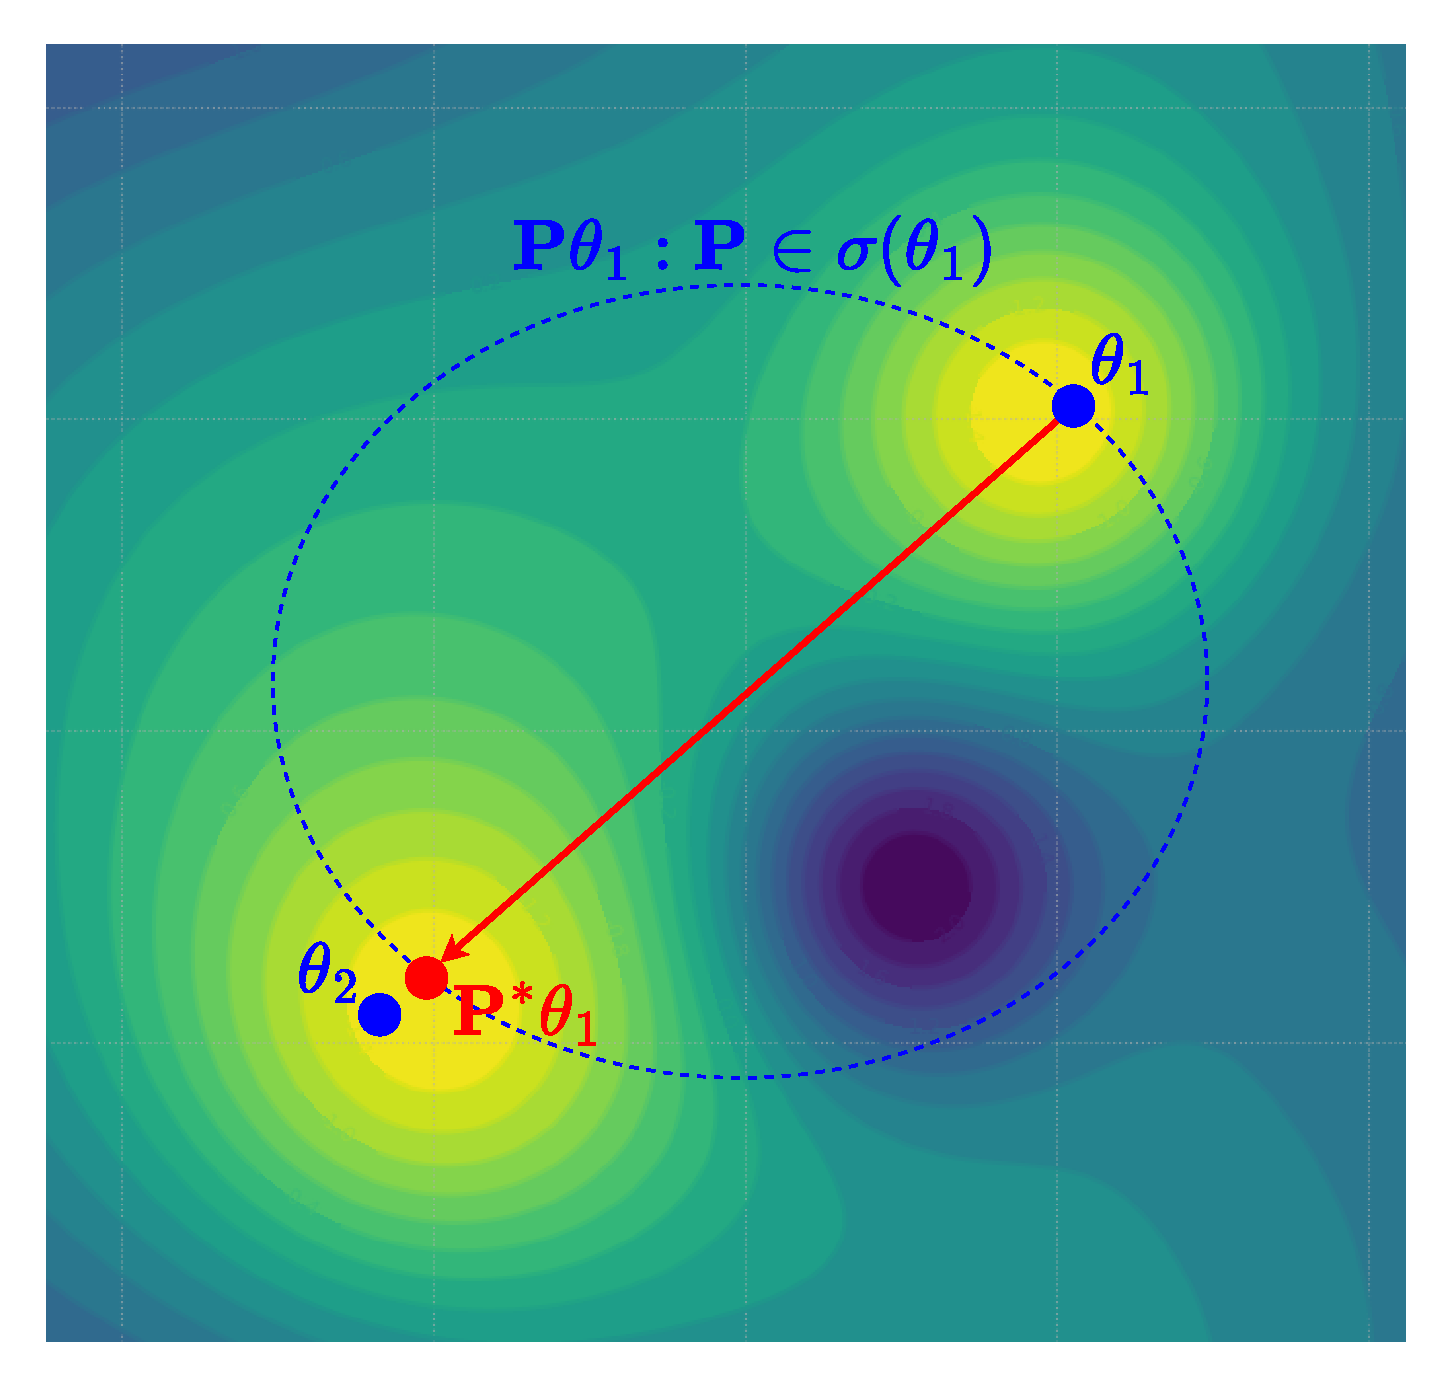
\includegraphics[width=0.6\textwidth]{figures/mode_connectivity.drawio.pdf}
    \caption{\label{fig:mode_conn} Mode connectivity.}    
\end{figure}


Closely related to the literature on symmetries of neural network weights is the topic of \textit{linear mode connectivity}, concerned with finding (linear) low-loss paths between SGD-optimized weights. Finding such paths is useful for many downstream applications, such as ensembling neural networks \citep{garipovLossSurfacesMode2018a} by finding accurate weights with different representations without training, or model merging \citep{stoicaZipItMergingModels2024}.

\citet{garipovLossSurfacesMode2018a} first formulated the problem as finding parametrized curves between NN weights, minimizing the loss across the curve. It was later conjectured by \citet{entezariRolePermutationInvariance2022} that up to permutation symmetries, such low-loss paths are linear. The linear mode connectivity hypothesis has since then given rise to a fruitful research area \citep{ferbachProvingLinearMode2024,rossiPermutationSymmetriesBayesian2023,zhaoUnderstandingModeConnectivity2023}. 

For our purposes, modes being linearly connected would imply that finding the optimal permutations could effectively reduce the number of modes in the weight-space posterior, making it easier to approximate. Accounting for this multi-modality has been shown to improve the effectiveness of Bayesian neural networks \citep{sommerConnectingDotsModeConnectedness2024}. With this motivation, we next focus on the literature around finding such permutations. 

\section{Aligning Neural Networks}

The problem of finding a permutation of one neural network weights to obtain a linear low-loss path with another neural network, we call \textit{aligning} neural networks, has given rise to a high number of methods over years, the entirety of which could be a thesis in itself. For instance, \citep{ainsworthGitReBasinMerging2023} propose various approaches. The first is a data-based approach that matches the activations of models $A$ and $B$ of each layer,
\begin{equation}
    \bP^* = \arg\min_{\bP \in S_d} \sum_{i=1}^n \Vert \mathbf{Z}_A - \bP \mathbf{Z}_B \Vert ^2
\end{equation}
with $d$ dimensional activations $\mathbf{Z}$ for $n$ data points. This is an instance of the \textit{linear assignment problem} which can be solved in polynomial time \citep{crouseImplementing2DRectangular2016}. An alternative is to align the weights of the neural networks directly, which can again be reduced to a linear assignment problem and is more efficient since it requires no forward passes over the model, but sacrifices accuracy by ignoring the data. 

\citet{penaReBasinImplicitSinkhorn2023} propose a more flexible framework, making it possible optimize for any differentiable objective, and we also use their approach in the rest of our work. \citet{penaReBasinImplicitSinkhorn2023} start by relaxing the constraint of binary permutation matrix $\bP \in \Pi$ to obtain unconstrained $\mathbf{X} \in \R^{m\times n}$. Such a matrix can then be mapped to the space of binary permutation matrices via the \textit{Sinkhorn operator}:
\begin{equation} \label{eq:sinkhorn}
    S_\tau(\mathbf{X}) = \arg\max_{\bP \in \Pi} \langle \bP, \mathbf{X} \rangle_F + \tau h(\bP)
\end{equation}
where $F$ denotes the Frobenius norm and entropy $h(\bP) = - \sum \bP \log \bP$. Then the optimization is performed over $\R^{m \times n}$, and a binary permutation matrix is obtained through the Sinkhorn operator. 

The main advantage of the approach of \citet{penaReBasinImplicitSinkhorn2023} is that it can be used with arbitrary differentiable objectives. To align the parameters $\theta_A$ and $\theta_B$, with $\pi_\bP$ denoting the permutation applied to the weights, \citet{penaReBasinImplicitSinkhorn2023} propose three objectives. First is a straightforward weight-matching similar to \citep{ainsworthGitReBasinMerging2023}
\begin{equation}
    \mathcal{L}_{L2} := \Vert \theta_A - \pi_\bP (\theta_B) \Vert^2,
\end{equation}
followed by two data-based objectives. Minimizing the mid-point loss between the two weights as
\begin{equation}
    \mathcal{L}_{\text{Mid}} := \mathcal{L} \left( \frac{\theta_A + \pi_\bP (\theta_B)}{2} \right) 
\end{equation}
or the loss at a random intermediate point 
\begin{equation}
    \mathcal{L}_{\text{Rnd}} := \mathcal{L} \left( (1-\lambda)\theta_A + \lambda \pi_\bP (\theta_B) \right) 
\end{equation}
with $\lambda \sim \mathcal{U}(0,1)$. At the end, particularly the data-based losses result in more effective permutations than the method of \citep{ainsworthGitReBasinMerging2023}, and we choose to use the approach of \citet{penaReBasinImplicitSinkhorn2023} in the rest of our work also considering its flexibility. 

\section{Canonical Representations of Neural Networks}

This discussion around permutation and scaling symmetries of neural networks culminates with \textit{canonical representations} of neural networks, i.e. unique representations for each set of permutation/scale-symmetric neural networks, limiting our discussion to ReLU networks for simplicity. Following the work of \citep{pittorinoDeepNetworksToroids2022}, this can achieved in two steps given a set of neural networks $\{ \theta_i\}_i^N$:
\begin{enumerate}
    \item Align all neural networks to a single \textit{reference} neural network $\theta'$, using the approach of \citep{penaReBasinImplicitSinkhorn2023}. 
    \item For each intermediate layer $l$ and neuron $k$, scale down the incoming weights and biases by the norm of the incoming weight vector, $\vert w_k^l \vert^{-1}$, and the outgoing weights by $\vert w_k^l \vert$. Additionally for classification tasks, normalize the last layer's weights to $\sqrt{C}$, with $C$ the number of classes. This does not change the predicted label due to the argmax operation at the last layer. 
\end{enumerate}
With these two operations, the permutation and scaling symmetries are ``broken,'' as all the neural networks that compute the same function up to permutation and scaling are now mapped to the same point in weight space. Nevertheless, while the scaling symmetry is broken exactly, the permutation symmetry is broken up to an approximation since the alignment methods \citep{ainsworthGitReBasinMerging2023,penaReBasinImplicitSinkhorn2023} only output approximate solutions. For this reason, as we will describe in the next section, we use graph neural networks to fully account for the permutation symmetries. This canonicalization also gives a specific geometric structure to the set of neural network weights. Each neuron, characterized by its incoming weights, now lies on the unit hypersphere, and each layer in turn has a product geometry of hyperspheres. This enables the computation of geodesic paths and distances between neural networks. 